\chapter{Physics objects and event reconstruction}
\label{chap:obj}
%Introduce reconstruction
The invisible Higgs analysis uses a wide range of objects from the jets and \MET that are present in the signal process, to charged leptons that are present in background processes. This range of objects means that information from all the CMS subdetectors must be used. The reconstruction of each physics object used from data collected by the CMS detector is described in this chapter, along with the overarching ``particle flow'' approach to data reconstruction used by CMS.

\section{Tracks}
\label{sec:tracks}
%This and next section from http://iopscience.iop.org/article/10.1088/1748-0221/9/10/P10009/pdf
The tracks reconstructed in the inner tracking detector of CMS are a key part of the reconstruction of most other objects used for physics analyses. For example the jet reconstruction algorithm combines information from the tracks and calorimeter energy deposits. The algorithm used by CMS is the Kalman filter based \ac{CTF}, which is described in \ReferenceRef{1748-0221-9-10-P10009}. 

The \ac{CTF} starts with seeds generated from either two or three hits in the pixel tracker. Seeds with two hits use the nominal crossing point of the beams to constrain the initial momentum of the track. The layers of the tracker are then iterated through, from inside to outside. The most compatible hit in each layer is added to the track and the track is refitted before moving to the next layer. Once the outside of the detector is reached the algorithm checks for tracks which share more than 19\% of their hits and discards the track with the fewest hits. In the case of the two tracks having an equal number of hits the track with the best fit, i.e. that having the lowest $\chi^{2}$, is kept. This process of reconstructing tracks starting from seeds is repeated up to six times, with hits associated to a successfully reconstructed track removed for the next iteration. 

After the full set of iterations is complete the tracks are refitted again using another Kalman filter, initialised with the innermost hit on the track and proceeding to iteratively add the hits on the track from inside to outside. This refitting aims to reduce biases from the track's seed including those introduced for two-hit seeds that include constraints from the beamspot. The refitted tracks are then smoothed by another Kalman filter, which is initialised with the current best-fit track hypothesis and iterates from the outside of the detector inwards. 

The smoothed tracks then have quality criteria, such as a requirement on the maximum number of layers the track traverses without leaving a hit, imposed to reject fake tracks. The efficiency of the \ac{CTF} is estimated in data using tracks from muons from Z decays, and is found to be greater than 99\% for muons with $1<\pt<100$ \GeV. For muons with $\pt=100 \GeV$ the \pt resolution of the \ac{CTF} is found to be approximately 2.8\%~\cite{1748-0221-9-10-P10009}.

\section{Primary vertex}
\label{sec:PV}
%Describe PV reconstruction
%Relevance to analysis
%Check if hard scatter defined elsewhere
The very high instantaneous luminosities present at the \LHC lead to a large probability of multiple proton-proton interactions occurring in each bunch crossing. It is therefore essential to identify the \ac{PV}, which relates to the highest energy interaction or ``hard scatter''. It is also useful to identify the \ac{PV} to distinguish ``prompt'' particles directly from the hard scatter from those resulting from processes which occur later such as heavy flavour hadron decay or photon conversion.

%Algorithm
The CMS \ac{PV} reconstruction algorithm has three steps, track selection, clustering of tracks into vertices and finally fitting the position of these vertices and is described in more detail in \ReferenceRef{1748-0221-9-10-P10009}. In the first step, track selection, the subset of tracks with non-significant transverse impact parameters is chosen. This selection removes tracks not coming from the primary interaction region.

The next step of clustering tracks into prototype vertices uses a \ac{DA} algorithm~\cite{DetAnnealing}. These prototype vertices then have their position determined by an adaptive vertex fitter~\cite{adaptivevertex}. This fitter starts by performing a fit to the position of the vertex, then assigning weights, $w_{i}$ to each track according to the probability that it belongs to the vertex, before repeating the process iteratively. Both of these algorithms also use the concept of ``cooling,'' where the algorithm is performed repeatedly as a temperature parameter, which controls the size of fluctuations around the current state of the system, is gradually reduced, to increase the chance of finding the global best fit solution.

The number of degrees of freedom of the resulting vertex is defined as:
\begin{equation}
  \label{eq:vertdof}
  n_{dof}=2\displaystyle\sum_{i=1}^{\# \rm{tracks}}w_i -3.
\end{equation}
This variable is highly correlated with the number of tracks compatible with the vertex and can therefore be used to select vertices coming from true proton-proton interactions.

The \ac{PV} is defined to be the vertex with the highest sum of the squared \pt of all the tracks contributing to it. If there is no reconstructed vertex the nominal beam crossing point is used. In the analyses described in this thesis events are required to have a real vertex, which has $n_{dof}>4$ and a maximum displacement in the $z$-direction ($xy$-plane) direction from the centre of the detector of 24 cm (2 cm).

%Performance, make sure jet is defined in theory section
The performance of the vertex reconstruction algorithm has been measured using events with at least one jet with $\pt>20$ GeV~\cite{1748-0221-9-10-P10009}. The efficiency to reconstruct at least one primary vertex in these events is found to be greater than 99\% for vertices with at least three tracks. The position resolution is found to vary as a function of the number of tracks associated to the vertex, being approximately 100\,\micron\, for vertices with 5 tracks and approaching 10\,\micron\, for vertices with greater than 50 tracks.

\section{Particle flow}
\label{sec:pf}
%Describe pf reconstruction, Relevance to analysis
\ac{PF} is an algorithm used by CMS to combine information from different sub-detectors into individual particles~\cite{CMS-PAS-PFT-09-001,CMS-PAS-PFT-10-001,CMS-PAS-PFT-10-002}. This approach is particularly beneficial for CMS as it allows the accurate momentum measurements of the inner tracker, and the excellent energy measurements and granularity of the \ac{ECAL} to be combined and used to improve the energy measurement of objects seen in the \ac{HCAL}. The \ac{PF}\,approach also allows calibrations specific to charged and neutral hadrons to be applied. The \ac{PF} algorithm classifies particles as charged hadrons, neutral hadrons, photons, muons and electrons. This set of particles, referred to as \ac{PF} candidates, can then further be used to calculate the \MET, as input to the jet reconstruction, for reconstructing taus and to calculate the isolation of leptons.

%Algorithm
The \ac{PF} algorithm starts with tracks, reconstructed as described in \SectionRef{sec:tracks}, and calorimeter clusters, which are reconstructed separately in each sub-detector of the calorimeter system. Clustering starts with seeds, which are the calorimeter cells which have the local maximum energy which is also more than twice the expected calorimeter noise, which is 80 (300) \MeV\, in the \ac{EB} (\ac{EE}) and 800\,\MeV\, in the \ac{HCAL}. Cells adjacent to the cluster are added if they also have energy more than twice the expected calorimeter noise. Cluster-track pairs whose cluster position and track trajectory are compatible are then linked together to identify charged particles. Linking between tracks from the inner tracker and the muon system is also performed to identify muons. The information from tracks with associated \ac{ECAL} clusters, i.e. those compatible with electrons, is further used to search for clusters compatible with having come from Bremsstrahlung photons from the electron; this is described further in \SectionRef{sec:electrons}.

Once electrons, muons and charged hadrons have been identified, further calorimeter clusters are identified as neutral hadrons or photons if they are in the \ac{HCAL} or \ac{ECAL} respectively. Excess energy in a calorimeter cluster compared to that expected from the associated tracks also allows the presence of neutral particles that would otherwise not have been identified to be determined.

\section{Electrons}
\label{sec:electrons}
%Describe electron reconstruction
As described in \SectionRef{sec:pf}, electrons are reconstructed by matching \ac{ECAL} deposits with tracks from the inner tracker. This process is complicated by the fact that electrons can lose significant amounts of energy, in the form of Bremsstrahlung photons, as they traverse the inner tracker. Approximately 35\% of electrons lose at least 70\% of their initial energy in this way~\cite{Baffioni:2006cd}. The Bremsstrahlung photons often convert to electron-positron pairs which are then further spread in the $\phi$ direction by CMS's solenoidal magnetic field. The electron reconstruction, which is described in detail in \ReferenceRef{1748-0221-10-06-P06005}, employs so-called ``supercluster'' algorithms to combine \ac{ECAL} deposits from both the initial electron and the Bremsstrahlung photons.

%supercluster forming and tracking
Due to their different geometries, different supercluster algorithms are used in the barrel and endcaps. In the barrel the ``hybrid'' clustering algorithm is used: this begins with a seed crystal which is the crystal with local maximum energy greater than 1 \GeV. Arrays of 5$\times$1 crystals in $\eta\times\phi$ are then added around the seed crystal if they are within 17 crystals of it in either direction in $\phi$ and have energy greater than 0.1 \GeV. Contiguous arrays are grouped into clusters. The final supercluster consists of all clusters from a seed with cluster energy greater than 0.35 \GeV.

In the endcap the ``multi-5$\times$5'' algorithm is used. This algorithm also starts with seed crystals, in this case those with energy higher than their four direct neighbours and also greater than 0.18 \GeV. Clusters are then made up of the 5$\times$5 square of crystals centered on the seed. Individual clusters whose seeds are within 0.07 in $\eta$ and 0.3 radians in $\phi$ of each other are grouped and kept as a supercluster if their total energy is greater than 1\GeV. A reference position for the supercluster is taken to be the energy-weighted average position of all the clusters belonging to it, and the maximum difference in $\phi$ between any cluster and the reference position is taken to be the size of the cluster in $\phi$. The individual clusters in a supercluster are then extrapolated to the preshower detector. Any preshower deposits within the supercluster's $\phi$ size plus 0.15 in $\phi$ and within $0.15$ in $\eta$ of a cluster in the supercluster are added to it.

The energy-weighted average position and energy of the final supercluster are then used to extrapolate the electron's track back to the innermost layers of the tracker for both electron charge hypotheses. This extrapolation is then matched to hits within a $\phi - z$ window of it, whose size is determined by the uncertainties on the $\phi$ position of the supercluster and the $z$ position of the beamspot. This size was typically 5 cm in 2012. This matched hit is used to update the estimated electron trajectory so that a hit in the second layer of the inner tracker can be searched for in a much narrower window. Hits in both the first and second layers compatible with a supercluster are then used as seeds for dedicated electron track reconstruction, performed using a \ac{GSF} algorithm~\cite{GSFalgorithm}, which performs better than a Kalman Filter for tracks with significant energy loss.

%ID
Electron identification criteria are applied to reject fake electrons caused by other particles such as pions. The variables used include:
\begin{itemize}
\item $\Delta\eta_{in}$ and $\Delta\phi_{in}$, which are the $\eta$ and $\phi$ distances between the electron track position extrapolated to the \ac{ECAL} and the supercluster position.
\item $\sigma_{i\eta i\eta}$, the energy-weighted $\eta$ width of the cluster.
\item $H/E$, the ratio between the energy deposited in the \ac{HCAL} and in the \ac{ECAL} in the region of the electron's seed cluster.
\end{itemize}
All of these variables are generally lower for real prompt electrons.

We also require the electrons to be isolated, i.e. have a low amount of other activity present around them in the detector. The variable used for this requirement is the effective area corrected \ac{PF} isolation, $I_{PF}$. In Run 1 it was defined as the sum of the \pt of the \ac{PF} candidates within a cone of $\Delta R<0.4$ around the direction of the electron, minus the expected contribution from \ac{PU} across the area of the electron.

%Performance
In the \ac{VBF} invisible Higgs boson decay searches described later in this thesis two sets of requirements on the above variables are used to identify electrons, both of which require that $|\eta|<2.4$. The ``veto'' set of identification criteria is looser and is used to veto events containing electrons. The other ``tight'' set of criteria is stricter and is used when we want to study events containing electrons. Tight electrons are required to be separated by more than 0.3 in $\Delta R$ from any veto muons to remove fake electrons from muons. The veto (tight) criteria have an efficiency of 93\% (85\%) for reconstructing central electrons with $\pt>50$ GeV~\cite{eleeff}. The veto (tight) electrons used in the analyses described in this thesis are required to have \pt$>10 (20)$ \GeV unless stated otherwise.

\section{Muons}
\label{sec:muons}
%Describe muon reconstruction %Relevance to analysis
Due to their relatively high mass and lack of strong force interactions, most muons deposit very little energy in the CMS calorimeters and thus leave the detector after passing through the muon system. As described in \SectionRef{sec:pf}, this means that muons can be reconstructed by searching for compatible tracks from the inner tracker and the muon system. The approach of requiring both inner tracker and muon system tracks greatly improves the discrimination between muons and hadronic activity and is referred to as ``global'' muon reconstruction.

%Algorithm
The CMS global muon reconstruction algorithm starts with each track in the muon system and searches for compatible tracks in the inner tracker ~\cite{MuonReco}. If a compatible inner tracker track is found, a track fit, similar to that described in section \SectionRef{sec:tracks}, is performed using the hits in both the inner tracker and muon system. The fit accounts for energy losses as the muon traverses the detector. It is found that for muons with $\pt>200$\GeV the global-muon fit is better than that from the tracker only~\cite{MuonReco}. However, due to the increased hadron discrimination described above all muons used for analyses in this thesis are required to have both inner tracker and muon system tracks. As with electrons it is also required that muons are isolated. The same isolation variable, $I_{PF}$, as described in \SectionRef{sec:electrons} is used for muon isolation. Global muon reconstruction is sufficient for use in vetoing events containing muons, and muons passing the above reconstruction are referred to as ``veto'' muons.

Where we want to study events containing muons, further identification criteria are used. This is because whilst global muon reconstruction removes most hadrons, some so-called ``punch through'' hadrons, which are energetic enough to travel all the way through the CMS calorimeters, can still be reconstructed as muons. Furthermore, it is desirable to separate real but non-prompt muons from hadron decay, from prompt muons from the hard scatter or tau decay. The identification consists of requiring a high quality global muon track fit, that the muon's track passes through at least 5 inner tracker layers, with at least one being a pixel layer, that the muon's track includes at least two hits in the muon system, and that there is at least one muon system track segment present. Muons passing these additional requirements are referred to as ``tight'' muons. In addition to the above requirements both veto and tight muons are required to have $|\eta|<2.1$.

%Performance
The efficiency of veto (tight) muon reconstruction has been found to be 98-99\% (96-98\%) depending on the $\eta$ of the muon, for muons with $\pt>10$\GeV~\cite{MuonReco}. This efficiency measurement was performed using events with $J/\psi$ or \PZ boson decays to muon pairs. The veto (tight) muons used in the analyses described in this thesis are required to have \pt$>10 (20)$ \GeV unless stated otherwise.

\section{Jets}
\label{sec:jets}
%Describe jet reconstruction %Relevance to analysis
As it is a hadron collider, quarks and gluons are very common at the \LHC. Furthermore, the presence of two final state quarks is one of the primary signatures of \ac{VBF} Higgs production, which is one of the main focuses of this thesis. Ascertaining the momentum of these strongly interacting particles is therefore very important. As discussed in \SectionRef{sec:higprod}, the hadronisation of strongly interacting particles results in highly collimated jets of particles. The momentum of the original parton which gave rise to the jet can be reconstructed by combining all of the particles in the resulting jet.

%Algorithm
%Performance

\subsection{Jet clustering}
\label{sec:jetclustering}
%IR and colinear safety and sequential recombination
Jet clustering algorithms take the many different types of particles that are expected to be present in the particle showers from hadronisation, and combine them into jets~\cite{Salam:2009jx}. It is important that jet clustering algorithms do not produce different reconstructed jets if a jet undergoes soft gluon radiation (called infrared unsafety) or if a gluon in it splits in two (called colinear unsafety). The algorithm used by CMS is a so-called sequential recombination algorithm. This class of algorithms requires a metric for calculating the distance between particles in the event, $d_{ij}$, and a metric for calculating the distance to a nominal beamline particle, $d_{iB}$ to be defined. The algorithms then proceed as follows:
\begin{itemize}
\item[1] Calculate the distance between all pairs of particles in the event including the nominal beamline.
\item[2] If the smallest distance is a $d_{ij}$ combine $i$ and $j$ together into a single new (pseudo-)particle and return to step 1.
\item[3] If the smallest distance is a $d_{iB}$, consider $i$ to be a final state jet and remove it from the list of particles. Return to step 1.
\item[4] Stop when no particles remain.
\end{itemize}

%anti-kt algorithm 
The particular algorithm used by CMS is the infrared and colinear safe anti-$k_{T}$ algorithm~\cite{1126-6708-2008-04-063}; its distances are defined as:
\begin{align}
d_{ij}&=\rm{min}\left(\mathit{p}_{\mathrm{T}\mathit{i}}^{-2},\mathit{p}_{\mathrm{T}\mathit{j}}^{-2}\right)\frac{\Delta \mathit{R}_{\mathit{ij}}^{2}}{\mathit{R}^{2}},\\
d_{iB}&=p_{T\mathit{i}}^{-2},
\end{align}
where $\Delta R_{ij}$ is the distance in the $\eta-\phi$ plane between particles $i$ and $j$ and $R$ is a parameter of the algorithm analogous to the maximum radius of the jet. This algorithm starts by clustering around the hardest particle in a region and therefore usually produces jets with circular cross-sections, with easy to calculate areas.

The anti-$k_{T}$ algorithm is implemented using the \textsc{FastJet} package~\cite{Cacciari:fastjet1} with the \ac{PF} candidates, described in \SectionRef{sec:pf}, used as input, the output jets are referred to as \ac{PF} jets. For analyses using data from \LHC Run 1 $R$ of 0.5 is used. In addition to these jets reconstructed from \ac{PF} candidates, in \ac{MC} events ``generator'' jets are also reconstructed by applying the anti-$k_{T}$ algorithm, with the same radius as that used for the \ac{PF} jets, to the final state particles produced by the generator before they are passed through the detector simulation.

\subsection{Jet identification}
\label{sec:jetid}
%PF , PU , and lepton cleaning ref previous sections
In order to reject jets that are badly reconstructed or just due to detector noise, identification criteria are imposed on the jets reconstructed by the above algorithm. These requirements are that:
\begin{itemize}
\item The jet contains at least two \ac{PF} candidates.
\item The total jet energy contribution from neutral hadrons must be less than 99\%.
\item The total jet energy contribution from photons must be less than 99\%.
\item The jet has contributions from both the \ac{ECAL} and \ac{HCAL}.
\item Jets with $\eta$ such that tracking information is available must have at least one charged object which contributes to the jet's energy and less than 99\% of their energy must be from electrons.
\end{itemize}
Real jets from quarks or gluons pass these requirements with over 99\% efficiency ~\cite{ARTICLE:CMSAN-14-227}.

In addition to jets from detector noise, it is also possible for the jet reconstruction to include particles that are not from the \ac{PV}, but instead come from \ac{PU} vertices. This can lead either to an overestimation of the energy of a real jet from the \ac{PV}, or to fake jets made up of energy from several vertices. The CMS pileup jet identification procedure~\cite{CMS-PAS-JME-13-005} combines several variables sensitive to the pileup contribution in a jet, such as information on how the \pt of the jet is shared between its constituents and the constituents' tracking information, into a \ac{BDT}~\cite{TMVA}. Simulated real jets from quarks pass this identification with 88-99\% efficiency depending on how central they are, while jets from pile-up are rejected with 40-87\% efficiency~\cite{CMS-PAS-JME-13-005}.

Jets are also required to have $\eta<4.7$ so that they are fully contained within the CMS detector. Finally, jets which are within 0.5 in the $\eta-\phi$ plane of any veto electron, defined in \SectionRef{sec:electrons}, or veto muon, defined in \SectionRef{sec:muons}, are vetoed, to avoid using jets which are due to misreconstructed leptons.

\subsection{Jet energy corrections}
\label{sec:jec}
%JEC
The energy of the jets clustered and identified by the CMS jet reconstruction often does not match the energy of the particle that initiated the jet. This can have many causes such as additional energy from \ac{PU}, miscalibration of the energy response of the calorimeters or energy deposited in uninstrumented areas of the detector. To account for these mismatches a correction to the jet energy is applied that has the following functional form and is described in detail in \ReferenceRef{CMS-JME-10-011}: 
\begin{equation}
  p_{\mu}^{\rm{cor}}=C_{\rm{offset}}\left(\pt^{\rm{raw}}\right)\cdot C_{\rm{rel}}\left(\eta\right)\cdot C_{\rm{abs}}\left(\pt'\right)\cdot C_{\rm{res}}\left(\pt'',\eta\right)\cdot p_{\mu}^{\rm{raw}}.
\end{equation}
Each $C$ in the equation represents a correction, $p_{\mu}^{\rm{cor}}$ is the corrected jet four-momentum, $p_{\mu}^{\rm{raw}}$ is the jet four-momentum before correction, $\pt'$ is the \pt after the offset and relative corrections, ($C_{\rm{offset}}$ and $C_{\rm{rel}}$) and $\pt''$ is the \pt after all but the residual correction ($C_{\rm{abs}}$).

The purpose of $C_{\rm{offset}}$ is to remove energy from the jet which is not due to activity from the \ac{PV} such as detector noise and \ac{PU}. The correction is calculated on a jet-by-jet basis by multiplying the median \pt density of the event in which the jet is by the jet's area. 

The relative correction, $C_{\rm{rel}}$, serves to make the jet energy response uniform in $\eta$. \ac{MC} truth information and the dijet \pt balance method, where the \pt of a well measured jet in the central region of the detector is compared to a second jet at a different $\eta$ in data events with only two jets, are used to calculate $C_{\rm{rel}}$.

The absolute correction $C_{\rm{abs}}$, makes the jet energy response uniform in \pt. As well as being calculated using \ac{MC} truth information, the correction is also calculated by using \PZ$/\gamma$+jets events, where the transverse momentum of the jets should balance the \PZ$/\gamma$. Both \PZ bosons that decay leptonically and photons have very good energy resolution, so any imbalances can be assumed to be due to jet mismeasurement.

Finally $C_{\rm{res}}$, which is applied only to data and not \ac{MC}, corrects for residual differences seen in both \pt and $\eta$ response between data and \ac{MC}. The total uncertainty on the overall jet energy correction is taken to be the sum in quadrature of the uncertainties on the individual corrections. The correction and its uncertainty are shown in \FigureRef{fig:jec}; the other two types of jets in the figure are not used in analyses described in this thesis and so are not discussed.

\begin{figure}
  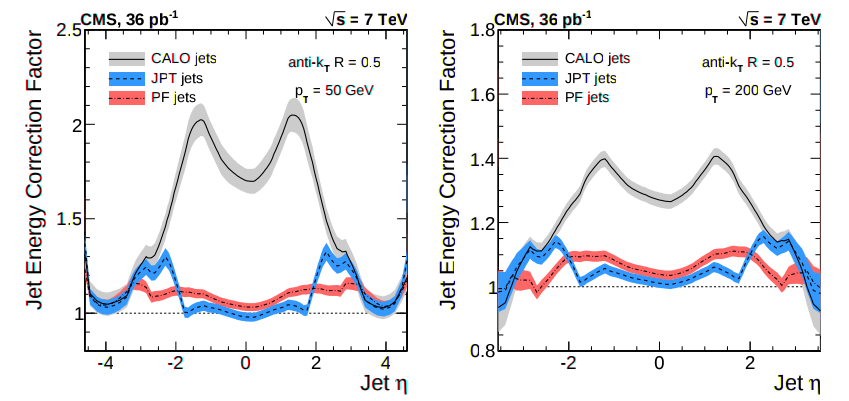
\includegraphics[width=1.2\largefigwidth]{plots/obj/jec.png}
  \caption[Total jet-energy-correction factor as a function of jet $\eta$ for jets with $\pt=50$\GeV\, (left) and $\pt=200$\GeV\, (right), for several types of jet reconstruction used at CMS. The bands indicate the corresponding uncertainty.]{Total jet-energy-correction factor as a function of jet $\eta$ for jets with $\pt=50$\GeV\, (left) and $\pt=200$\GeV\, (right), for several types of jet reconstruction used at CMS. The bands indicate the corresponding uncertainty~\cite{CMS-JME-10-011}.}
  \label{fig:jec}
\end{figure}
\section{Missing transverse energy}
\label{sec:MET}
%Describe MET reconstruction
Particles which interact only weakly with normal matter, such as neutrinos and hypothetical \ac{DM} particles, will pass through the CMS detector without interacting. The only signature that they leave is a momentum imbalance between the visible particles in an event. The initial transverse momentum of the colliding protons is low (less than a \ac{GeV}), so any significant imbalance can be interpreted as evidence for non-interacting particles. The high hermeticity of the CMS detector allows this imbalance, the \MET, first described in \SectionRef{sec:higprod}, to be measured accurately. As the analyses described in this thesis are searches for invisibly decaying Higgs bosons, the measurement of \MET is crucial.

%Algorithm
The CMS \MET reconstruction algorithm defines \MET as the negative vectorial sum of the \pt of all \ac{PF} candidates~\cite{CMS-PAS-JME-12-002}. For processes such as \PZ boson decays to muon pairs, or $\gamma$+jets, there should be no \MET as all the decay products are visible. However, as can be seen from \FigureRef{fig:metresponse}, these events often still appear to have \MET due to the resolution of the \pt measurements of the various objects making up the \ac{PF} candidates, primarily the jets which are numerous and do not have as good resolution as other objects.

\begin{figure}
  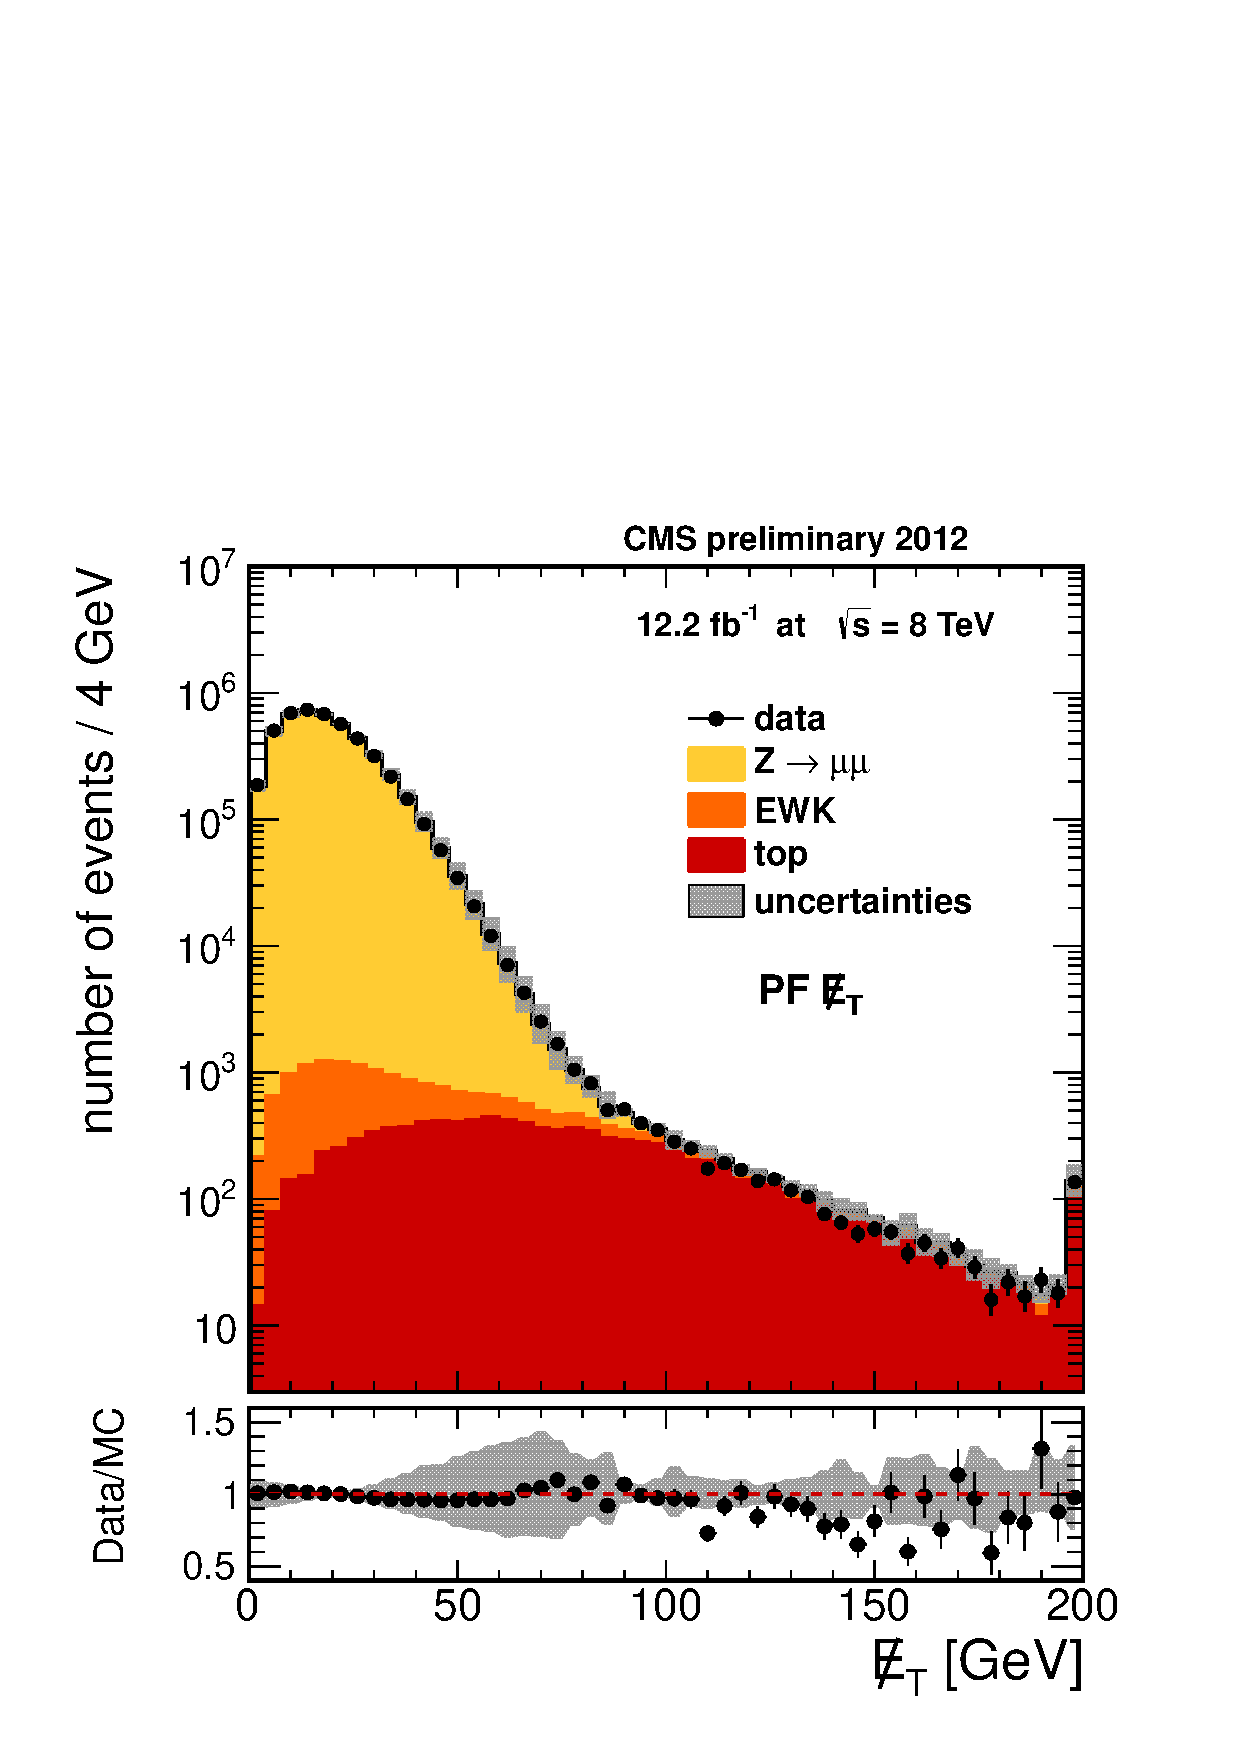
\includegraphics[width=0.6\largefigwidth]{plots/obj/metzmumu.pdf}
  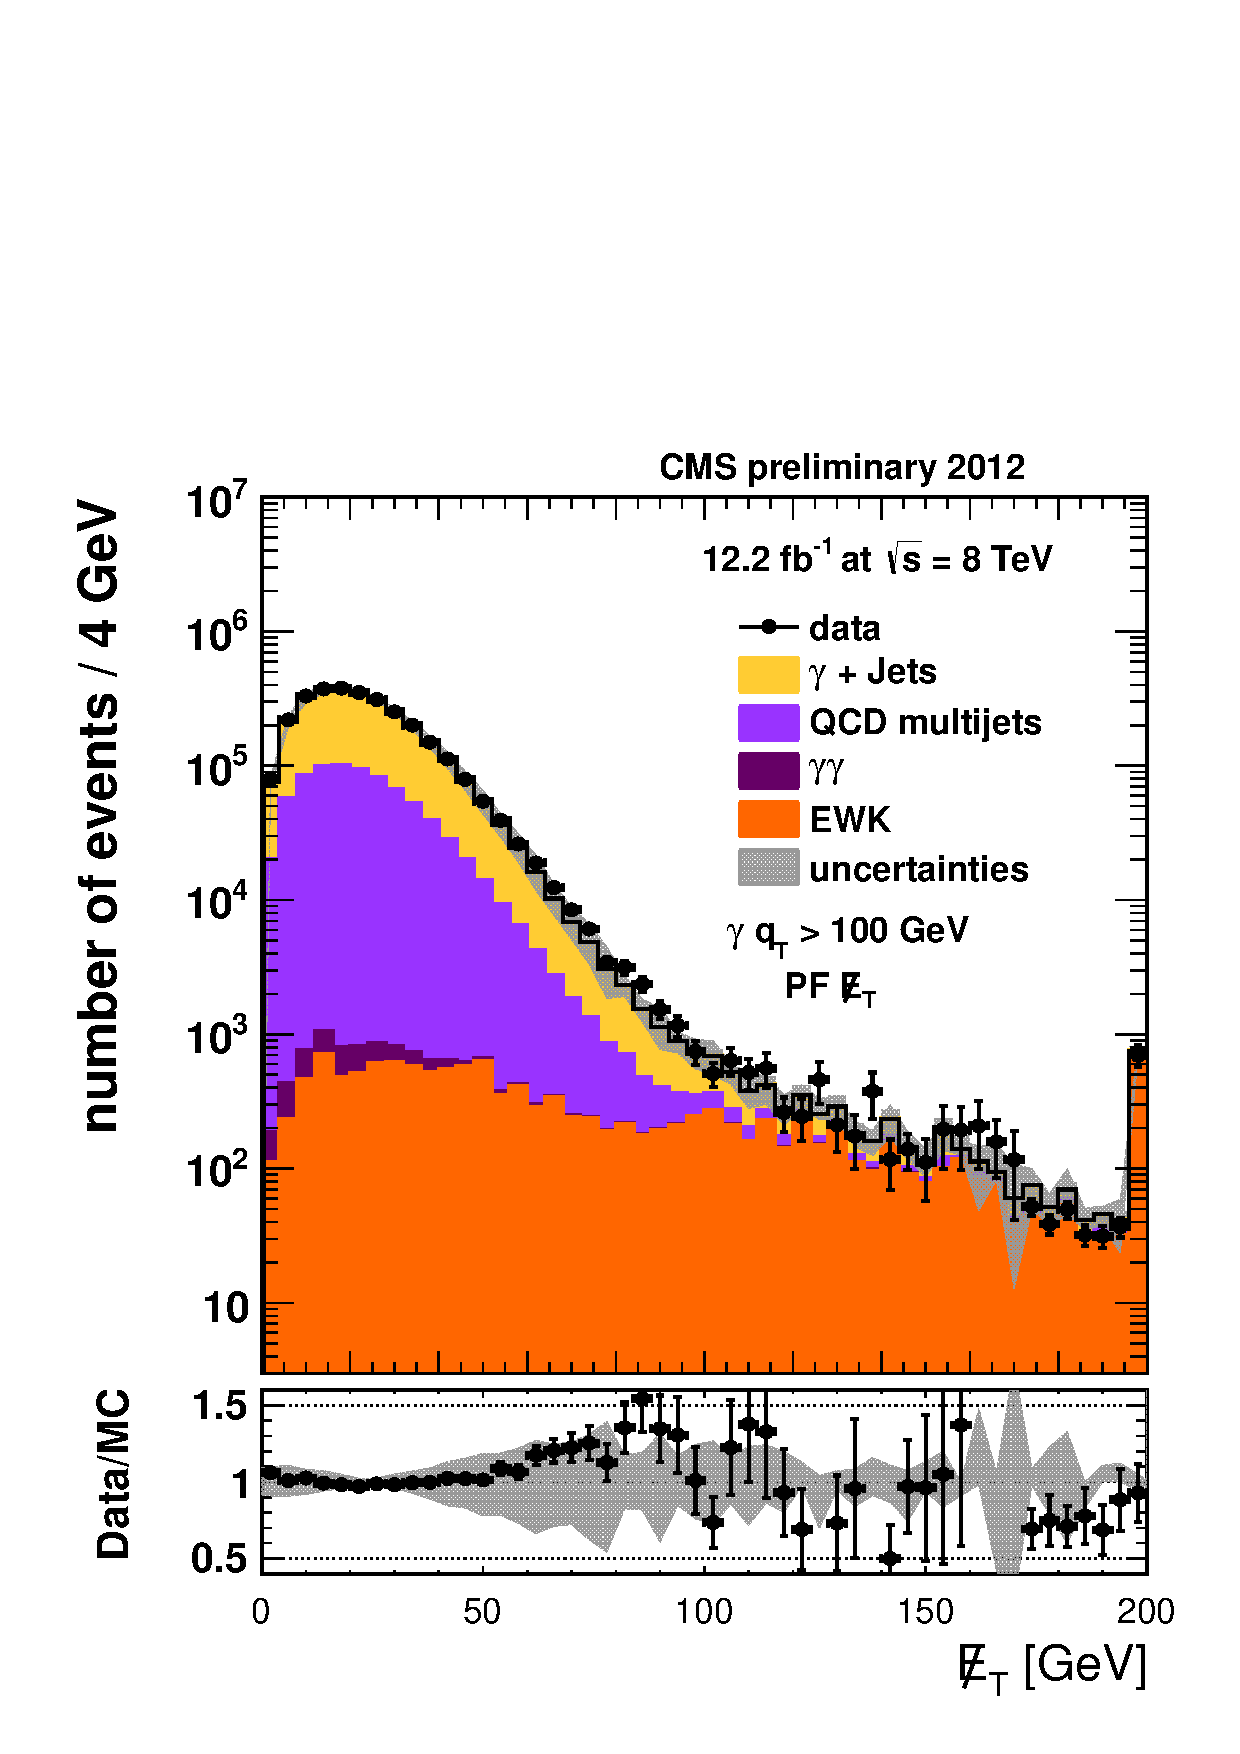
\includegraphics[width=0.6\largefigwidth]{plots/obj/metgammajets.pdf}
  \caption[Distributions of the uncorrected \MET in $\PZ\rightarrow\mu\mu$ events (left) and $\gamma$+jets events (right) in $\sqrt{s}=8$\TeV\, data and simulation. The shaded band corresponds to the systematic uncertainty.]{Distributions of the uncorrected \MET in $\PZ\rightarrow\mu\mu$ events (left) and $\gamma$+jets events (right) in $\sqrt{s}=8$\TeV\, data and simulation. The shaded band corresponds to the systematic uncertainty~\cite{CMS-PAS-JME-12-002}.}
  \label{fig:metresponse}
\end{figure}

The jet energy corrections, described in \SectionRef{sec:jec}, alter the energy of jets, and in doing so alter the total energy present in the event. These changes are propagated to the \MET. Furthermore, as charged particle flow candidates can be determined to be from the \ac{PV} or a \ac{PU} vertex it is also possible to correct the \MET for \ac{PU} contributions. This correction uses the ratio of the energy response of CMS for charged and neutral particles to estimate the neutral \ac{PU} contribution from the charged \ac{PU} contribution.

In addition to the above corrections, filters are applied to reject events where detector or beam effects lead to a high probability of spurious \MET. Examples of the effects which are removed with these filters include particles directly hitting the photodetectors in the \ac{ECAL} or significant energy deposits from the halo of particles surrounding the \LHC beam.

%METNOMU
In the \ac{VBF} invisible Higgs boson decay searches described below events with \PW or \PZ boson decays to muons are used to estimate the rate of some background processes. As part of this estimation the muons from the \PW or \PZ boson decays are ignored when calculating the \MET. The variable \METnoMU, which is the \MET calculated ignoring all tight muons, is used for this estimation.
\section{Taus}
\label{sec:taus}
%Describe tau reconstruction %Relevance to analysis
Approximately 35\% of taus decay to lighter charged leptons and neutrinos~\cite{pdg}. In this case, due to the short lifetime of the tau, the resulting charged leptons are reconstructed as prompt electrons or muons and the neutrinos cause \MET, therefore no specific tau reconstruction is necessary. However, the other $\sim$65\% of tau decays are so-called hadronic tau decays, where the decay products are hadrons and a tau neutrino. This section will describe the reconstruction of these tau decays.

%Algorithm
CMS uses the so-called \ac{HPS} algorithm for reconstructing hadronic tau decays, described in detail in \ReferenceRef{CMS-PAS-TAU-11-001}. Almost all hadronic tau decay modes consist of one or three charged hadrons and up to two neutral pions~\cite{pdg}. The \ac{HPS} algorithm aims to reconstruct both the charged hadrons and the photons which result from the neutral pion decays.

The \ac{HPS} algorithm is seeded by a \ac{PF} jet, described in \SectionRef{sec:jets}, and starts by creating a ``strip'' with the four-momentum of the most energetic \ac{EM} \ac{PF} candidate, i.e. photon or electron, in the jet. Other \ac{EM} candidates are then searched for within  a window of 0.05 (0.2) in $\eta$ ($\phi$) of the strip's centre. The most energetic particle that is found is added to the strip and the four-momentum is updated. This process is repeated until no more particles are found, and if the strip has \pt$>1$\GeV\, at this point it is kept. Combinations of charged hadrons and strips consistent with tau decay modes are then searched for, and if one is found the resulting combination is taken to be a hadronic tau.

Taus are required to be isolated. The isolation is calculated as the sum of all hadronic and photon \ac{PF} candidates from the \ac{PV} within a cone of size $\Delta R=0.5$ of the tau. \ac{PF} candidates not compatible with the \ac{PV} within 0.8 in $R$ of the tau are used to estimate and correct for the contribution to the isolation from \ac{PU}. 

Electrons which emit Bremsstrahlung photons can look very much like one charged hadron plus a neutral pion. A \ac{BDT} is trained, using similar variables to those used for the electron identification in \SectionRef{sec:electrons}, to remove these particles. Taus that are consistent with being from a muon are also rejected. This rejection is performed by requiring that the tau is not reconstructed as a track compatible with hits in the muon system. The final efficiency of the CMS hadronic tau reconstruction for taus with \pt$>20$ \GeV is found to be 55\%, with a fake rate of 2 (3)\% for non-hadronic tau objects to be reconstructed as hadronic taus in the barrel (endcap) region of the detector.

\section{MC weights}
\label{sec:mcweights}
As discussed in \SectionRef{sec:sim} proton-proton collisions at the \LHC are simulated using \ac{MC} generators. In some cases the results of these simulations need to be modified to better match the observed data, by ``weighting'' the \ac{MC} events. One example of this is cross-section weighting, where a weight is applied to account for the difference between the number of events generated and that expected to be observed in data for a given integrated luminosity. Further weights are applied to correct the generated distribution of the number of primary vertices to match that in data (called pileup reweighting), to account for differences between the simulated lepton identification efficiency and that observed in data, and to correct the generated \pt spectrum of top quarks to better match that observed in data.
